% The farmer's problem: land allocation, cattle feed, and market flows.
%
% Birge & Louveaux, "Introduction to Stochastic Programming", 2nd ed., Sec. 1.1a,
% pp. 4-5 (PDF viewer p. 31 carries printed folio 5, so in Ch. 1
% printed = viewer - 26). The book states the problem and Table 1 but draws NO
% figure; the diagram is Prof. Dowling's own, hand-drawn on p. 1 of the Fall
% 2018 Lecture 21 scan.
%
% SINGLE SOURCE. This file is \input by
%   optimization-private/lecture-notes/lectures/stochastic-programming-intro.tex
% via \figsrc, and `make' renders ../media/figures/farmer-crop-allocation.{png,svg}
% for the website, where notebooks/4/SP.ipynb displays the PNG. Handout, website
% and notebook therefore cannot drift.
%
% CONVERGED 2026-08-22 (JUDGEMENT_CALLS.md item H1). Until then the same diagram
% was drawn TWICE: this file, which only the website showed, and a separate
% inline tikzpicture in the lecture, which only the handout showed. They were not
% equivalent. This drawing is the UNION of the two:
%   * from this file    the horizontal layout, the "(acres)" units, and the
%                       cattle-feed arrows out to the animals -- which the
%                       inline version omitted entirely
%   * from the lecture  the "farm (land)" / "market" labels of the scan, and the
%                       solid-vs-dashed encoding that separates sales from
%                       purchases by line style as well as by direction
% Two things were also corrected on the way: the feed arrows read ">= 200 T" and
% ">= 240 T", because B&L p. 4 says "at least 200 tons (T) of wheat and 240 T of
% corn are needed for cattle feed" and the lecture writes the constraint as an
% inequality; and the crop is "sugar beets", matching B&L Table 1 and the lecture
% prose, not the bare "Beets" this file used to print.
%
% WHY HORIZONTAL, when the 2018 scan is vertical (farm above, market below). Not
% taste: the cattle-feed arrows are the reason. Stacking the crops puts a free
% left edge on each crop's own row, so the wheat and corn feed arrows leave from
% the rows they belong to. In the scan's vertical layout the crops sit side by
% side, so an arrow out of the wheat CELL would have to cross the corn and sugar
% beet cells to reach anything drawn beside the farm. Horizontal is the only
% orientation that carries all three flows -- sales, purchases and feed --
% without a crossing.
%
% Greyscale: black line art, nothing encoded by hue, so it is identical in print.
% Sales vs purchases is carried twice over, by arrow direction AND by
% solid-vs-dashed, which is what "redundant encoding" means here. Same house
% precedent as scenario-tree.tex in this directory.
%
% Base TikZ only -- no library beyond what `tikz' itself provides ("stealth" is
% a base arrow tip). Nothing here needs arrows.meta or positioning, so this file
% compiles under the lecture preamble and the figures/ preamble alike.
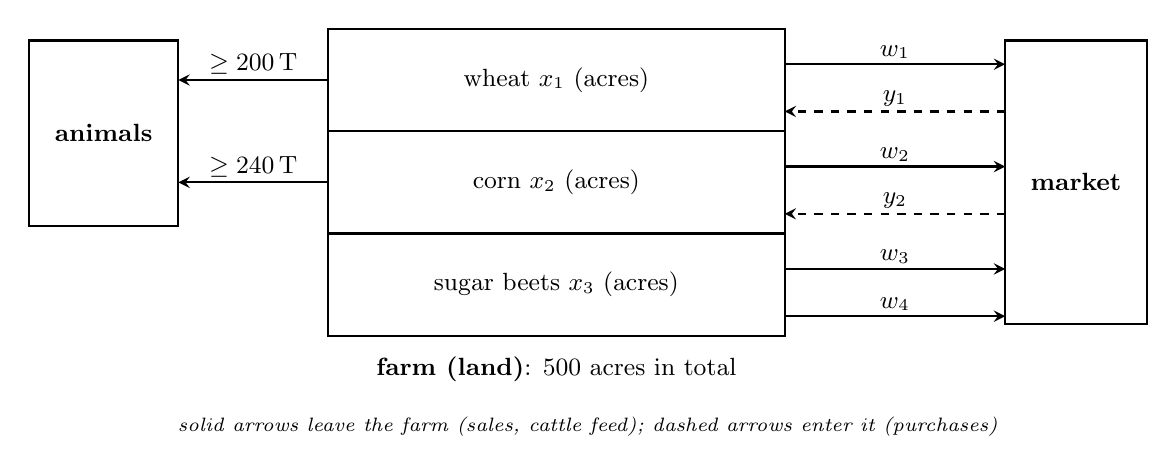
\begin{tikzpicture}[>=stealth, font=\small,
    flow/.style={->, thick},
    buy/.style={->, thick, dashed},
    lab/.style={midway, above, inner sep=1.5pt, font=\small}]

% ---------------- the farm: three crop rows, one per stage-1 variable
  \draw[thick] (0,0) rectangle (5.8,3.9);
  \draw[thick] (0,1.3) -- (5.8,1.3);
  \draw[thick] (0,2.6) -- (5.8,2.6);
  \node at (2.9,3.25) {wheat $x_1$ (acres)};
  \node at (2.9,1.95) {corn $x_2$ (acres)};
  \node at (2.9,0.65) {sugar beets $x_3$ (acres)};
  \node at (2.9,-0.42) {\textbf{farm (land)}: 500 acres in total};

% ---------------- the market
  \draw[thick] (8.6,0.15) rectangle (10.4,3.75);
  \node at (9.5,1.95) {\textbf{market}};

% ---------------- the animals: the cattle-feed requirement
  \draw[thick] (-3.8,1.4) rectangle (-1.9,3.75);
  \node at (-2.85,2.575) {\textbf{animals}};

% ---------------- sales: farm -> market, solid, one arrow per sales variable.
% Each arrow sits INSIDE its crop's row, so w_3 and w_4 visibly both come out of
% sugar beets: the two beet prices are one crop sold two ways.
  \draw[flow] (5.8,3.45) -- (8.6,3.45) node[lab] {$w_1$};
  \draw[flow] (5.8,2.15) -- (8.6,2.15) node[lab] {$w_2$};
  \draw[flow] (5.8,0.85) -- (8.6,0.85) node[lab] {$w_3$};
  \draw[flow] (5.8,0.25) -- (8.6,0.25) node[lab] {$w_4$};

% ---------------- purchases: market -> farm, dashed. Only wheat and corn; the
% farmer never buys sugar beets, which is why there is no third dashed arrow.
  \draw[buy] (8.6,2.85) -- (5.8,2.85) node[lab] {$y_1$};
  \draw[buy] (8.6,1.55) -- (5.8,1.55) node[lab] {$y_2$};

% ---------------- cattle feed: farm -> animals, the minimum requirement
  \draw[flow] (0,3.25) -- (-1.9,3.25) node[lab] {$\ge 200$\,T};
  \draw[flow] (0,1.95) -- (-1.9,1.95) node[lab] {$\ge 240$\,T};

% ---------------- legend, so the line-style encoding travels with the drawing
  \node[font=\scriptsize\itshape, align=center] at (3.3,-1.15)
    {solid arrows leave the farm (sales, cattle feed);
     dashed arrows enter it (purchases)};
\end{tikzpicture}
